\section*{Tests}
\label{sec:tests}

\subsection*{Correctness Tests}\label{subsec:correctness_tests}
The correctness suite resides in
\texttt{CHC-Verification/correctness\_tests/} and is executed with
\texttt{pytest} over \texttt{unittest.TestCase}-based test classes. The fixture set includes 64 \texttt{.tl} programs across the three modes, covering a wide range of semantic properties and edge cases. These fixtue programs can be found in \texttt{CHC-Verification/correctness\_tests/programs/}.

\subsubsection*{Evaluation modules and responsibilities}

\begin{longtable}{p{0.20\textwidth} p{0.80\textwidth}}
\toprule
\textbf{File} & \textbf{Role in evaluation} \\
\midrule
\texttt{test\_default.py} & Validates concrete-start-state verification in \texttt{default} mode, including arithmetic, geometric, pen-state, directional, heading-grid, trigonometric, and nested-loop behaviors. \\
\texttt{test\_specific.py} & Validates parameterized initialization in \texttt{specific} mode, with boundary-sensitive outcomes under user-supplied parameter dictionaries. \\
\texttt{test\_universal.py} & Validates symbolic/unconstrained initialization in \texttt{universal} mode, API-level validation errors, heading-grid handling, and terminating-scope properties. \\
\texttt{helpers.py} & Shared harness for loading programs, invoking \texttt{CHC\_Verification}, building assertion contexts, and standardizing property checks. \\
\texttt{README.md} & Documents suite structure, mode coverage, fixture list, and execution commands. \\
\bottomrule
\end{longtable}

\subsubsection*{Coverage snapshot}

\begin{itemize}[leftmargin=1.5em]
	\item Total collected correctness tests: \textbf{206}
	\item Mode split: \textbf{48} (default), \textbf{70} (specific), \textbf{90} (universal)
	\item Fixture programs in \texttt{programs/}: \textbf{64} \texttt{.tl} files
	\item Explicitly skipped tests: \textbf{6} timeout-marked heading/trig-heavy scenarios
\end{itemize}

\subsubsection*{Category coverage across modes}

\begin{itemize}[leftmargin=1.5em]
	\item \textbf{Default mode:} arithmetic invariants, geometric bounds, pen-state properties, directional/heading checks, and advanced nested control-flow fixtures.
	\item \textbf{Specific mode:} same semantic families under concrete parameter assignments, including multi-parameter and chained-update programs.
	\item \textbf{Universal mode:} unconstrained initial-state reasoning, relational arithmetic properties, API-validation behavior, and terminating-scope checks.
\end{itemize}

\subsubsection*{How to run}

\textbf{From repository root (recommended):}
\begin{lstlisting}[style=terminal, language=bash]
cd Chiron-Framework/ChironCore
source .venv/bin/activate
cd ../../CHC-Verification/correctness_tests
pytest -q
\end{lstlisting}

\textbf{Useful variants:}
\begin{lstlisting}[style=terminal, language=bash]
# verbose mode
pytest -v

# collect-only sanity check
pytest --collect-only -q

# run one mode file
pytest test_default.py -q

# run one test class
pytest test_specific.py::TestSpecificArithmetic -q

# run one test case
pytest test_universal.py::TestUniversalAPI::test_invalid_mode_error -q
\end{lstlisting}

\subsection*{Performance Tests}
\label{sec:performance_tests}

The CHC verification pipeline is benchmarked to stress-test solver scalability under various optimization levels. 
The test suite resides in \noindent\textit{\small Folder: \texttt{CHC-Verification/performance\_tests}} and is executed with \texttt{pytest} using \texttt{pytest-xdist} for parallel execution.
The fixture contains 21 \texttt{.tl} programs across the three modes and cover cases that can blow up the number of solver constraints. 
The fixture programmes can be found in \noindent\textit{\small Folder: \texttt{CHC-Verification/performance\_tests/programs/}}.


\subsubsection*{Test Infrastructure}

The performance test suite is built on Python's \texttt{unittest} framework and reuses the shared helper infrastructure from Milestone~1. Each test case runs the verification pipeline across six configurations: three optimization levels (\texttt{NONE}, \texttt{BASIC}, \texttt{AGGRESSIVE}) combined with two hint modes (no hint, with hint).

\begin{longtable}{p{0.28\textwidth} p{0.66\textwidth}}
\toprule
\textbf{File} & \textbf{Purpose} \\
\midrule
\texttt{tests/test\_default.py} & Performance benchmarks in \texttt{default} mode, testing loop scaling, nesting depth, wide state, branching density, trigonometric motion, and property complexity. \\
\texttt{tests/test\_universal.py} & Performance benchmarks in \texttt{universal} mode with unconstrained initial states. \\
\texttt{tests/test\_specific.py} & Performance benchmarks in \texttt{specific} mode using explicit parameter assignments. \\
\texttt{tests/helpers.py} & Extended test infrastructure supporting timing measurements across all six configurations and CSV output generation. \\
\texttt{perf\_results\_*.csv} & Raw timing data output files containing build times, solve times, and verdicts for each test case. \\
\bottomrule
\end{longtable}


The benchmark suite comprises 129 test cases distributed across three verification modes and six property categories.

\begin{table}[H]
\centering
\caption{Test case distribution by category and verification mode.}
\label{tab:test-distribution}
\begin{tabular}{lcccc}
\toprule
\textbf{Category} & \textbf{Default} & \textbf{Universal} & \textbf{Specific} & \textbf{Total} \\
\midrule
Loop Scaling      & 12 & 12 & 15 & 39 \\
Nesting Depth     &  6 &  8 & 10 & 24 \\
Wide State        &  5 &  7 & 10 & 22 \\
Branching         &  5 &  6 &  9 & 20 \\
Trigonometric     &  6 &  5 &  8 & 19 \\
Heading/Turns     &  5 &  0 &  0 &  5 \\
\midrule
\textbf{Total}    & \textbf{39} & \textbf{38} & \textbf{52} & \textbf{129} \\
\bottomrule
\end{tabular}
\end{table}


\subsubsection*{Benchmark Programs}

The performance suite includes 21 benchmark programs organized into six categories:

\begin{longtable}{p{0.24\textwidth} p{0.70\textwidth}}
\toprule
\textbf{Program file} & \textbf{Purpose in evaluation} \\
\midrule
\multicolumn{2}{l}{\textit{Loop Scaling (testing solver performance as loop iterations increase)}} \\
\midrule
\texttt{perf\_repeat\_10.tl} & Simple accumulator loop with 10 iterations; baseline for loop scaling. \\
\texttt{perf\_repeat\_50.tl} & Same accumulator with 50 iterations; tests medium-scale loop invariants. \\
\texttt{perf\_repeat\_100.tl} & Same accumulator with 100 iterations; tests large-scale loop invariants. \\
\midrule
\multicolumn{2}{l}{\textit{Nesting Depth (testing nested loop invariant synthesis)}} \\
\midrule
\texttt{perf\_deep\_nest\_3.tl} & Three-level nested loops ($4^3 = 64$ total iterations); produces chained counters $a$, $b$, $c$. \\
\texttt{perf\_deep\_nest\_4.tl} & Four-level nested loops ($3^4 = 81$ total iterations); adds counter $d$ for deeper invariants. \\
\midrule
\multicolumn{2}{l}{\textit{Wide State (testing high-dimensional state tracking)}} \\
\midrule
\texttt{perf\_wide\_vars.tl} & Eight chained variables updated per iteration; tests 8-dimensional arithmetic invariants. \\
\midrule
\multicolumn{2}{l}{\textit{Branching Density (testing branching CFG complexity)}} \\
\midrule
\texttt{perf\_many\_branches.tl} & Six-iteration loop with four sequential if/else blocks per iteration; dense branching. \\
\midrule
\multicolumn{2}{l}{\textit{Trigonometric Motion (testing heading-dependent position updates)}} \\
\midrule
\texttt{perf\_trig\_10.tl} & \texttt{forward 10; right 90} repeated 10 times; tests trigonometric constraint scaling. \\
\texttt{perf\_trig\_20.tl} & Same motion pattern repeated 20 times; harder trigonometric reasoning. \\
\midrule
\multicolumn{2}{l}{\textit{Heading/Turns (testing heading normalization cost)}} \\
\midrule
\texttt{perf\_turns\_20.tl} & \texttt{right 345} repeated 20 times; heading visits only $\{0, 345\}$. \\
\texttt{perf\_turns\_50.tl} & Same turn pattern repeated 50 times; tests grid-check scaling. \\
\bottomrule
\end{longtable}

%% =============================================================================
\subsubsection*{Aggregate Results by Mode and Configuration}
%% =============================================================================

Tables~\ref{tab:agg-default}, \ref{tab:agg-universal}, and \ref{tab:agg-specific} present aggregate results for each verification mode across all six configurations.

\begin{table}[H]
\centering
\caption{Aggregate results: \textbf{Default} mode (39 test cases).}
\label{tab:agg-default}
\begin{tabular}{lcccccc}
\toprule
\textbf{Config} & \textbf{Passed} & \textbf{Failed} & \textbf{Skipped} & \textbf{Completion} & \textbf{Avg Build (s)} & \textbf{Avg Solve (s)} \\
\midrule
NONE       & 15 &  0 & 24 & 38.5\% & 0.141 & 2.74 \\
BASIC      & 23 &  0 & 16 & \textbf{59.0\%} & 0.100 & 2.16 \\
AGGRESSIVE & 15 &  0 & 24 & 38.5\% & 0.114 & 3.03 \\
NONE+H     & 23 &  0 & 16 & \textbf{59.0\%} & 0.122 & 2.23 \\
BASIC+H    & 23 &  0 & 16 & \textbf{59.0\%} & 0.094 & 2.21 \\
AGGRESSIVE+H & 23 &  0 & 16 & \textbf{59.0\%} & 0.123 & 2.40 \\
\bottomrule
\end{tabular}
\end{table}

\begin{table}[H]
\centering
\caption{Aggregate results: \textbf{Universal} mode (38 test cases).}
\label{tab:agg-universal}
\begin{tabular}{lcccccc}
\toprule
\textbf{Config} & \textbf{Passed} & \textbf{Failed} & \textbf{Skipped} & \textbf{Completion} & \textbf{Avg Build (s)} & \textbf{Avg Solve (s)} \\
\midrule
NONE       & 26 &  0 & 12 & 68.4\% & 0.206 & 4.51 \\
BASIC      & 34 &  0 &  4 & 89.5\% & 0.863 & 4.15 \\
AGGRESSIVE & 24 &  0 & 14 & 63.2\% & 0.175 & 2.11 \\
NONE+H     & 30 &  0 &  8 & 78.9\% & 0.172 & 1.76 \\
BASIC+H    & 36 &  0 &  2 & \textbf{94.7\%} & 0.715 & 4.49 \\
AGGRESSIVE+H & 31 &  0 &  7 & 81.6\% & 0.170 & 2.60 \\
\bottomrule
\end{tabular}
\end{table}

\begin{table}[H]
\centering
\caption{Aggregate results: \textbf{Specific} mode (52 test cases).}
\label{tab:agg-specific}
\begin{tabular}{lcccccc}
\toprule
\textbf{Config} & \textbf{Passed} & \textbf{Failed} & \textbf{Skipped} & \textbf{Completion} & \textbf{Avg Build (s)} & \textbf{Avg Solve (s)} \\
\midrule
NONE       & 13 &  0 & 39 & 25.0\% & 0.312 & 1.09 \\
BASIC      & 18 &  0 & 34 & 34.6\% & 0.262 & 1.19 \\
AGGRESSIVE & 13 &  0 & 39 & 25.0\% & 0.322 & 1.33 \\
NONE+H     & 20 &  0 & 32 & \textbf{38.5\%} & 0.281 & 1.74 \\
BASIC+H    & 19 &  0 & 33 & 36.5\% & 0.246 & 2.09 \\
AGGRESSIVE+H & 19 &  0 & 33 & 36.5\% & 0.283 & 2.22 \\
\bottomrule
\end{tabular}
\end{table}

Figure~\ref{fig:verdict-stacked} provides a visual comparison of verdict distributions across all modes and configurations.

\begin{figure}[H]
\centering
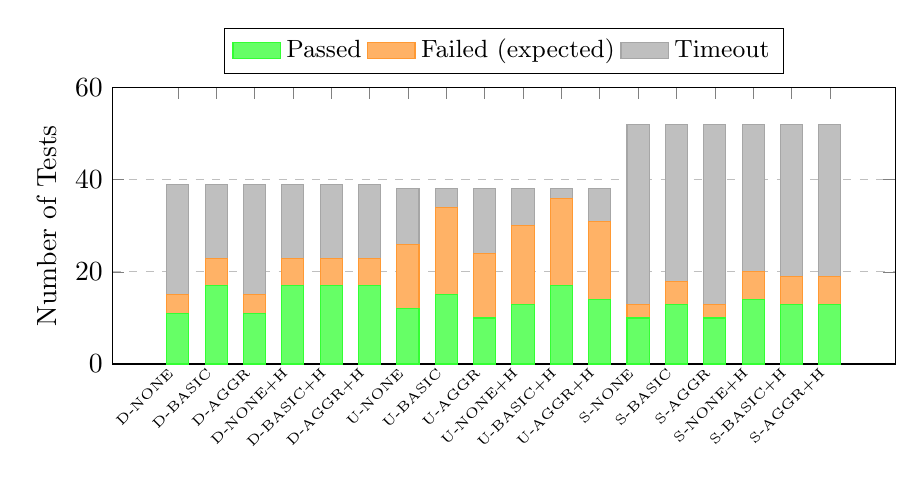
\begin{tikzpicture}
\begin{axis}[
    ybar stacked,
    width=0.95\linewidth,
    height=0.42\linewidth,
    bar width=8pt,
    ymajorgrids=true,
    grid style=dashed,
    ylabel={Number of Tests},
    symbolic x coords={D-NONE,D-BASIC,D-AGGR,D-NONE+H,D-BASIC+H,D-AGGR+H,
                       U-NONE,U-BASIC,U-AGGR,U-NONE+H,U-BASIC+H,U-AGGR+H,
                       S-NONE,S-BASIC,S-AGGR,S-NONE+H,S-BASIC+H,S-AGGR+H},
    xtick=data,
    x tick label style={rotate=45, anchor=east, font=\tiny},
    legend style={at={(0.5,1.05)}, anchor=south, legend columns=3, font=\small},
    ymin=0, ymax=60,
    area legend
]

% Passed (green)
\addplot[fill=green!60, draw=green!80] coordinates {
    (D-NONE,11) (D-BASIC,17) (D-AGGR,11) (D-NONE+H,17) (D-BASIC+H,17) (D-AGGR+H,17)
    (U-NONE,12) (U-BASIC,15) (U-AGGR,10) (U-NONE+H,13) (U-BASIC+H,17) (U-AGGR+H,14)
    (S-NONE,10) (S-BASIC,13) (S-AGGR,10) (S-NONE+H,14) (S-BASIC+H,13) (S-AGGR+H,13)
};
\addlegendentry{Passed}

% Failed (orange)
\addplot[fill=orange!60, draw=orange!80] coordinates {
    (D-NONE,4) (D-BASIC,6) (D-AGGR,4) (D-NONE+H,6) (D-BASIC+H,6) (D-AGGR+H,6)
    (U-NONE,14) (U-BASIC,19) (U-AGGR,14) (U-NONE+H,17) (U-BASIC+H,19) (U-AGGR+H,17)
    (S-NONE,3) (S-BASIC,5) (S-AGGR,3) (S-NONE+H,6) (S-BASIC+H,6) (S-AGGR+H,6)
};
\addlegendentry{Failed (expected)}

% Unknown/Timeout (gray)
\addplot[fill=gray!50, draw=gray!70] coordinates {
    (D-NONE,24) (D-BASIC,16) (D-AGGR,24) (D-NONE+H,16) (D-BASIC+H,16) (D-AGGR+H,16)
    (U-NONE,12) (U-BASIC,4) (U-AGGR,14) (U-NONE+H,8) (U-BASIC+H,2) (U-AGGR+H,7)
    (S-NONE,39) (S-BASIC,34) (S-AGGR,39) (S-NONE+H,32) (S-BASIC+H,33) (S-AGGR+H,33)
};
\addlegendentry{Timeout}

\end{axis}
\end{tikzpicture}
\caption{Verdict distribution across all modes (D=Default, U=Universal, S=Specific) and configurations. Green indicates proven properties, orange indicates expected counterexamples found, gray indicates solver timeout.}
\label{fig:verdict-stacked}
\end{figure}

%% =============================================================================
\subsubsection*{Timing Results}
%% =============================================================================

Table~\ref{tab:timing-default}, Table~\ref{tab:timing-universal}, and Table~\ref{tab:timing-specific} present detailed timing results for each mode tests using the best available configuration.

{\small
\begin{longtable}{p{0.12\textwidth} p{0.14\textwidth} p{0.16\textwidth} c c r r r}
\caption{Solver timing benchmark: Default mode (best optimisation per property).}
\label{tab:timing-default} \\
\toprule
\textbf{Program} & \textbf{Optimisation} & \textbf{Property} & \textbf{Verdict} & \textbf{Result} & \textbf{Build (s)} & \textbf{Solve (s)} & \textbf{Total (s)} \\
\midrule
\endfirsthead
\toprule
\textbf{Program} & \textbf{Optimisation} & \textbf{Property} & \textbf{Verdict} & \textbf{Result} & \textbf{Build (s)} & \textbf{Solve (s)} & \textbf{Total (s)} \\
\midrule
\endhead
\midrule
\endfoot
\bottomrule
\endlastfoot
%% Loop Scaling Properties
\multicolumn{8}{l}{\textit{Default mode -- Loop Scaling Properties}} \\
\midrule
\texttt{repeat\_10}  & BASIC       & $x \geq 0$             & True  & Passed &  0.022 &  0.026 &  0.048 \\
\texttt{repeat\_10}  & NONE        & $x \leq 10$            & True  & Passed &  0.053 &  6.547 &  6.600 \\
\texttt{repeat\_10}  & NONE        & $x$ violated           & False & Passed &  0.031 &  1.774 &  1.805 \\
\texttt{repeat\_10}  & AGGRESSIVE  & single atom            & True  & Passed &  0.038 &  0.104 &  0.142 \\
\texttt{repeat\_10}  & AGGRESSIVE  & two atom conj          & True  & Passed &  0.033 & 12.588 & 12.621 \\
\texttt{repeat\_10}  & BASIC+H     & exact disj 11          & True  & Passed &  0.024 & 10.285 & 10.309 \\
\texttt{repeat\_50}  & AGGRESSIVE  & $x \geq 0$             & True  & Passed &  0.020 &  0.004 &  0.023 \\
\texttt{repeat\_50}  & NONE        & $x \leq 50$            & --    & Skipped&  0.030 & 60.011 & \textit{timeout} \\
\texttt{repeat\_50}  & NONE        & $x$ violated           & False & Passed &  0.062 &  0.970 &  1.032 \\
\texttt{repeat\_100} & BASIC       & $x \geq 0$             & True  & Passed &  0.014 &  0.004 &  0.018 \\
\texttt{repeat\_100} & NONE        & $x \leq 100$           & --    & Skipped&  0.027 & 60.011 & \textit{timeout} \\
\texttt{repeat\_100} & NONE        & $x$ violated           & False & Passed &  0.051 &  0.863 &  0.914 \\
\midrule
%% Nesting Depth Properties
\multicolumn{8}{l}{\textit{Default mode -- Nesting Depth Properties}} \\
\midrule
\texttt{deep\_nest\_3} & AGGRESSIVE & all $\geq 0$  & True  & Passed &  0.159 &  0.034 &  0.194 \\
\texttt{deep\_nest\_3} & BASIC      & $c$ tight     & --    & Skipped&  0.207 & 60.012 & \textit{timeout} \\
\texttt{deep\_nest\_3} & BASIC+H    & $c$ violated  & --    & Skipped&  0.211 & 60.039 & \textit{timeout} \\
\texttt{deep\_nest\_4} & BASIC      & all $\geq 0$  & True  & Passed &  0.252 &  0.034 &  0.286 \\
\texttt{deep\_nest\_4} & NONE       & $d$ tight     & --    & Skipped&  0.270 & 60.020 & \textit{timeout} \\
\texttt{deep\_nest\_4} & NONE       & $d$ violated  & --    & Skipped&  0.292 & 60.007 & \textit{timeout} \\
\midrule
%% Wide State Properties
\multicolumn{8}{l}{\textit{Default mode -- Wide State Properties}} \\
\midrule
\texttt{wide\_vars} & NONE+H       & all positive  & False & Passed &  0.435 &  0.151 &  0.586 \\
\texttt{wide\_vars} & AGGRESSIVE+H & $a$ tight     & --    & Skipped&  0.341 & 60.054 & \textit{timeout} \\
\texttt{wide\_vars} & NONE         & $a$ violated  & --    & Skipped&  0.242 & 60.018 & \textit{timeout} \\
\texttt{wide\_vars} & NONE         & $h \geq 0$    & --    & Skipped&  0.249 & 60.007 & \textit{timeout} \\
\texttt{wide\_vars} & AGGRESSIVE+H & $h$ tight     & --    & Skipped&  0.302 & 60.056 & \textit{timeout} \\
\midrule
%% Branching Properties
\multicolumn{8}{l}{\textit{Default mode -- Branching Properties}} \\
\midrule
\texttt{many\_branches} & NONE    & $x \geq 0$    & True  & Passed &  0.270 &  0.105 &  0.375 \\
\texttt{many\_branches} & BASIC   & acc $\geq 0$  & True  & Passed &  0.197 &  0.081 &  0.278 \\
\texttt{many\_branches} & BASIC   & $x$ tight     & --    & Skipped&  0.136 & 60.011 & \textit{timeout} \\
\texttt{many\_branches} & BASIC   & $x$ violated  & --    & Skipped&  0.137 & 60.011 & \textit{timeout} \\
\texttt{many\_branches} & NONE+H  & acc violated  & --    & Skipped&  0.176 & 60.031 & \textit{timeout} \\
\midrule
%% Trigonometric Properties
\multicolumn{8}{l}{\textit{Default mode -- Trigonometric Properties}} \\
\midrule
\texttt{trig\_10}  & BASIC   & heading quarters       & True  & Passed &  0.083 &  0.389 &  0.472 \\
\texttt{trig\_10}  & BASIC+H & pen up                 & True  & Passed &  0.083 &  0.135 &  0.217 \\
\texttt{trig\_10}  & BASIC+H & $\mathit{ycor} \geq 0$ & False & Passed &  0.049 &  0.433 &  0.481 \\
\texttt{trig\_20}  & BASIC   & heading quarters       & True  & Passed &  0.081 &  0.215 &  0.296 \\
\texttt{trig\_20}  & BASIC   & pen up                 & True  & Passed &  0.076 &  0.062 &  0.138 \\
\texttt{trig\_20}  & BASIC   & $\mathit{ycor} \geq 0$ & False & Passed &  0.068 &  0.822 &  0.890 \\
\midrule
%% Heading/Turns Properties
\multicolumn{8}{l}{\textit{Default mode -- Heading/Turns Properties}} \\
\midrule
\texttt{turns\_20} & BASIC   & heading binary   & --    & Skipped&  0.030 & 60.014 & \textit{timeout} \\
\texttt{turns\_20} & BASIC+H & heading grid 24  & True  & Passed &  0.037 &  0.098 &  0.136 \\
\texttt{turns\_20} & BASIC   & heading $\geq 0$ & True  & Passed &  0.029 &  0.048 &  0.077 \\
\texttt{turns\_50} & BASIC+H & heading binary   & --    & Skipped&  0.037 & 60.123 & \textit{timeout} \\
\texttt{turns\_50} & BASIC+H & heading $\geq 0$ & True  & Passed &  0.017 &  0.041 &  0.058 \\
\end{longtable}
}

{\small
\begin{longtable}{p{0.12\textwidth} p{0.14\textwidth} p{0.16\textwidth} c c r r r}
\caption{Solver timing benchmark: Universal mode (best optimisation per property).}
\label{tab:timing-universal} \\
\toprule
\textbf{Program} & \textbf{Optimisation} & \textbf{Property} & \textbf{Verdict} & \textbf{Result} & \textbf{Build (s)} & \textbf{Solve (s)} & \textbf{Total (s)} \\
\midrule
\endfirsthead
\toprule
\textbf{Program} & \textbf{Optimisation} & \textbf{Property} & \textbf{Verdict} & \textbf{Result} & \textbf{Build (s)} & \textbf{Solve (s)} & \textbf{Total (s)} \\
\midrule
\endhead
\midrule
\endfoot
\bottomrule
\endlastfoot
%% Loop Scaling Properties
\multicolumn{8}{l}{\textit{Universal mode -- Loop Scaling Properties}} \\
\midrule
\texttt{repeat\_10}  & BASIC        & $x$ nonneg all   & False & Passed &  0.013 &  0.005 &  0.018 \\
\texttt{repeat\_10}  & BASIC        & $x$ nonneg term  & True  & Passed &  0.007 &  0.005 &  0.013 \\
\texttt{repeat\_10}  & BASIC        & $x$ violated     & False & Passed &  0.006 &  0.007 &  0.013 \\
\texttt{repeat\_10}  & BASIC        & $x$ tight        & True  & Passed &  0.006 &  0.006 &  0.012 \\
\texttt{repeat\_50}  & AGGRESSIVE   & $x$ nonneg all   & False & Passed &  0.023 &  0.011 &  0.033 \\
\texttt{repeat\_50}  & AGGRESSIVE+H & $x$ nonneg       & True  & Passed &  0.015 &  0.015 &  0.030 \\
\texttt{repeat\_50}  & BASIC        & $x$ tight        & True  & Passed &  0.027 &  0.006 &  0.033 \\
\texttt{repeat\_50}  & BASIC        & $x$ violated     & False & Passed &  0.024 &  0.021 &  0.044 \\
\texttt{repeat\_100} & NONE         & $x$ nonneg all   & False & Passed &  0.027 &  0.008 &  0.036 \\
\texttt{repeat\_100} & AGGRESSIVE+H & $x$ nonneg term  & True  & Passed &  0.017 &  0.022 &  0.039 \\
\texttt{repeat\_100} & BASIC        & $x$ violated     & False & Passed &  0.042 &  0.004 &  0.045 \\
\texttt{repeat\_100} & BASIC        & $x$ tight        & True  & Passed &  0.039 &  0.015 &  0.054 \\
\midrule
%% Nesting Depth Properties
\multicolumn{8}{l}{\textit{Universal mode -- Nesting Depth Properties}} \\
\midrule
\texttt{deep\_nest\_3} & BASIC    & $c$ nonneg    & False & Passed &  0.299 &  0.021 &  0.320 \\
\texttt{deep\_nest\_3} & BASIC+H  & all nonneg    & True  & Passed &  0.235 &  0.163 &  0.398 \\
\texttt{deep\_nest\_3} & BASIC+H  & $c$ tight     & True  & Passed &  0.223 &  2.265 &  2.488 \\
\texttt{deep\_nest\_3} & BASIC+H  & $c$ violated  & False & Passed &  0.226 &  2.286 &  2.512 \\
\texttt{deep\_nest\_4} & BASIC    & $d$ nonneg    & False & Passed &  0.517 &  0.060 &  0.577 \\
\texttt{deep\_nest\_4} & BASIC+H  & all nonneg    & True  & Passed &  0.381 & 22.157 & 22.537 \\
\texttt{deep\_nest\_4} & BASIC    & $d$ tight     & --    & Skipped&  0.369 & 60.023 & \textit{timeout} \\
\texttt{deep\_nest\_4} & BASIC+H  & $d$ violated  & False & Passed &  0.433 & 28.591 & 29.024 \\
\midrule
%% Wide State Properties
\multicolumn{8}{l}{\textit{Universal mode -- Wide State Properties}} \\
\midrule
\texttt{wide\_vars} & AGGRESSIVE+H & all positive (F) & False & Passed &  0.285 &  0.059 &  0.344 \\
\texttt{wide\_vars} & AGGRESSIVE   & all positive (P) & True  & Passed &  0.322 &  0.323 &  0.645 \\
\texttt{wide\_vars} & AGGRESSIVE   & $a$ tight        & True  & Passed &  0.270 &  0.070 &  0.340 \\
\texttt{wide\_vars} & NONE         & $a$ violated     & False & Passed &  0.273 &  0.082 &  0.355 \\
\texttt{wide\_vars} & NONE         & $h$ nonneg       & True  & Passed &  0.274 &  0.121 &  0.395 \\
\texttt{wide\_vars} & AGGRESSIVE   & $h$ tight        & True  & Passed &  0.292 &  0.106 &  0.398 \\
\texttt{wide\_vars} & NONE         & $h$ violated     & False & Passed &  0.336 &  0.196 &  0.532 \\
\midrule
%% Branching Properties
\multicolumn{8}{l}{\textit{Universal mode -- Branching Properties}} \\
\midrule
\texttt{many\_branches} & AGGRESSIVE   & $x$ nonneg   & False & Passed &  0.174 &  0.019 &  0.193 \\
\texttt{many\_branches} & NONE+H       & acc nonneg   & True  & Passed &  0.208 &  0.190 &  0.398 \\
\texttt{many\_branches} & BASIC        & acc nonneg   & False & Passed &  0.211 &  0.163 &  0.374 \\
\texttt{many\_branches} & AGGRESSIVE+H & $x$ violated & False & Passed &  0.239 & 30.238 & 30.477 \\
\texttt{many\_branches} & NONE         & acc violated & --    & Skipped&  0.185 & 60.022 & \textit{timeout} \\
\texttt{many\_branches} & NONE         & $x$ tight    & True  & Passed &  0.177 & 34.987 & 35.164 \\
\end{longtable}
}

{\small
\begin{longtable}{p{0.12\textwidth} p{0.14\textwidth} p{0.16\textwidth} c c r r r}
\caption{Solver timing benchmark: Specific mode (best optimisation per property).}
\label{tab:timing-specific} \\
\toprule
\textbf{Program} & \textbf{Optimisation} & \textbf{Property} & \textbf{Verdict} & \textbf{Result} & \textbf{Build (s)} & \textbf{Solve (s)} & \textbf{Total (s)} \\
\midrule
\endfirsthead
\toprule
\textbf{Program} & \textbf{Optimisation} & \textbf{Property} & \textbf{Verdict} & \textbf{Result} & \textbf{Build (s)} & \textbf{Solve (s)} & \textbf{Total (s)} \\
\midrule
\endhead
\midrule
\endfoot
\bottomrule
\endlastfoot
%% Loop Scaling Properties
\multicolumn{8}{l}{\textit{Specific mode -- Loop Scaling Properties}} \\
\midrule
\texttt{s\_repeat\_50}  & AGGRESSIVE   & $x$ nonneg       & True  & Passed &  0.033 &  0.009 &  0.042 \\
\texttt{s\_repeat\_50}  & BASIC        & $x$ viol offset  & False & Passed &  0.023 &  0.037 &  0.060 \\
\texttt{s\_repeat\_50}  & AGGRESSIVE   & $x$ tight        & --    & Skipped&  0.038 & 60.011 & \textit{timeout} \\
\texttt{s\_repeat\_50}  & NONE         & $x$ tight offset & --    & Skipped&  0.051 & 60.011 & \textit{timeout} \\
\texttt{s\_repeat\_50}  & AGGRESSIVE+H & $x$ violated     & --    & Skipped&  0.061 & 60.030 & \textit{timeout} \\
\texttt{s\_repeat\_100} & AGGRESSIVE   & $x$ nonneg       & True  & Passed &  0.033 &  0.008 &  0.041 \\
\texttt{s\_repeat\_100} & AGGRESSIVE   & single atom      & True  & Passed &  0.060 &  0.086 &  0.146 \\
\texttt{s\_repeat\_100} & NONE+H       & exact disj 101   & --    & Skipped&  0.030 & 60.058 & \textit{timeout} \\
\texttt{s\_repeat\_100} & NONE+H       & tight shifted    & --    & Skipped&  0.027 & 60.017 & \textit{timeout} \\
\texttt{s\_repeat\_100} & NONE         & two atom conj    & --    & Skipped&  0.054 & 60.027 & \textit{timeout} \\
\midrule
%% Nesting Depth Properties
\multicolumn{8}{l}{\textit{Specific mode -- Nesting Depth Properties}} \\
\midrule
\texttt{s\_nest\_3} & BASIC        & all nonneg       & True  & Passed &  0.187 &  0.038 &  0.225 \\
\texttt{s\_nest\_3} & NONE         & $c$ tight        & --    & Skipped&  0.210 & 60.012 & \textit{timeout} \\
\texttt{s\_nest\_3} & AGGRESSIVE+H & $c$ tight offset & --    & Skipped&  0.330 & 60.045 & \textit{timeout} \\
\texttt{s\_nest\_3} & NONE         & $c$ violated     & --    & Skipped&  0.254 & 60.013 & \textit{timeout} \\
\texttt{s\_nest\_3} & AGGRESSIVE   & $c$ viol offset  & --    & Skipped&  0.243 & 60.015 & \textit{timeout} \\
\texttt{s\_nest\_4} & NONE         & all nonneg       & True  & Passed &  0.653 &  0.253 &  0.906 \\
\texttt{s\_nest\_4} & NONE         & $d$ tight        & --    & Skipped&  0.369 & 60.016 & \textit{timeout} \\
\texttt{s\_nest\_4} & NONE         & $d$ tight offset & --    & Skipped&  0.387 & 60.014 & \textit{timeout} \\
\texttt{s\_nest\_4} & AGGRESSIVE+H & $d$ violated     & --    & Skipped&  0.534 & 60.062 & \textit{timeout} \\
\texttt{s\_nest\_4} & AGGRESSIVE+H & $d$ viol offset  & --    & Skipped&  0.583 & 60.048 & \textit{timeout} \\
\midrule
%% Wide State Properties
\multicolumn{8}{l}{\textit{Specific mode -- Wide State Properties}} \\
\midrule
\texttt{s\_wide} & AGGRESSIVE   & all positive (P)   & True  & Passed &  0.206 &  0.091 &  0.297 \\
\texttt{s\_wide} & AGGRESSIVE+H & all positive (F)   & False & Passed &  0.305 &  0.135 &  0.439 \\
\texttt{s\_wide} & NONE         & chain all pos      & True  & Passed &  0.239 &  0.103 &  0.342 \\
\texttt{s\_wide} & NONE         & $a$ violated       & False & Passed &  0.181 & 12.916 & 13.097 \\
\texttt{s\_wide} & AGGRESSIVE+H & $a$ tight          & --    & Skipped&  0.245 & 60.047 & \textit{timeout} \\
\texttt{s\_wide} & NONE         & $h$ nonneg         & --    & Skipped&  0.238 & 60.018 & \textit{timeout} \\
\texttt{s\_wide} & AGGRESSIVE   & $h$ tight          & --    & Skipped&  0.260 & 60.015 & \textit{timeout} \\
\texttt{s\_wide} & NONE         & $h$ tight zero     & --    & Skipped&  0.226 & 60.019 & \textit{timeout} \\
\texttt{s\_wide} & AGGRESSIVE   & $h$ violated       & --    & Skipped&  0.222 & 60.018 & \textit{timeout} \\
\texttt{s\_wide} & NONE         & $h$ viol zero      & --    & Skipped&  0.247 & 60.017 & \textit{timeout} \\
\midrule
%% Branching Properties
\multicolumn{8}{l}{\textit{Specific mode -- Branching Properties}} \\
\midrule
\texttt{s\_branches} & NONE+H       & acc nonneg (1) & True  & Passed &  0.652 &  0.142 &  0.794 \\
\texttt{s\_branches} & AGGRESSIVE   & acc nonneg (2) & True  & Passed &  0.580 &  0.097 &  0.677 \\
\texttt{s\_branches} & BASIC        & $x$ nonneg     & True  & Passed &  0.621 &  0.152 &  0.773 \\
\texttt{s\_branches} & BASIC+H      & acc tight (1)  & --    & Skipped&  0.623 & 60.045 & \textit{timeout} \\
\texttt{s\_branches} & AGGRESSIVE+H & acc tight (2)  & --    & Skipped&  0.555 & 60.042 & \textit{timeout} \\
\texttt{s\_branches} & AGGRESSIVE+H & acc violated(1)& --    & Skipped&  0.577 & 60.043 & \textit{timeout} \\
\texttt{s\_branches} & BASIC        & acc violated(2)& --    & Skipped&  0.585 & 60.019 & \textit{timeout} \\
\texttt{s\_branches} & AGGRESSIVE+H & $x$ tight      & --    & Skipped&  0.568 & 60.041 & \textit{timeout} \\
\texttt{s\_branches} & BASIC+H      & $x$ violated   & --    & Skipped&  0.581 & 60.063 & \textit{timeout} \\
\midrule
%% Trigonometric Properties
\multicolumn{8}{l}{\textit{Specific mode -- Trigonometric Properties}} \\
\midrule
\texttt{s\_trig\_10} & BASIC        & heading quarters (1) & True  & Passed &  0.184 &  0.548 &  0.732 \\
\texttt{s\_trig\_10} & AGGRESSIVE+H & heading quarters (2) & True  & Passed &  0.141 &  0.632 &  0.773 \\
\texttt{s\_trig\_10} & BASIC        & pen up               & True  & Passed &  0.111 &  0.202 &  0.313 \\
\texttt{s\_trig\_10} & BASIC        & $\mathit{ycor}$ (1)  & False & Passed &  0.122 &  0.958 &  1.080 \\
\texttt{s\_trig\_10} & BASIC        & $\mathit{ycor}$ (2)  & False & Passed &  0.110 &  1.890 &  2.000 \\
\texttt{s\_trig\_20} & BASIC+H      & heading quarters     & True  & Passed &  0.120 &  1.438 &  1.557 \\
\texttt{s\_trig\_20} & BASIC        & pen up               & True  & Passed &  0.111 &  0.113 &  0.224 \\
\texttt{s\_trig\_20} & NONE+H       & $\mathit{ycor}$      & False & Passed &  0.242 &  1.515 &  1.757 \\
\end{longtable}
}

%% =============================================================================
\subsubsection*{Build Time Analysis Across Verification Modes}
%% =============================================================================

Figure~\ref{fig:build-time-modes} shows average build times across the three verification modes for each configuration.

\begin{figure}[H]
\centering
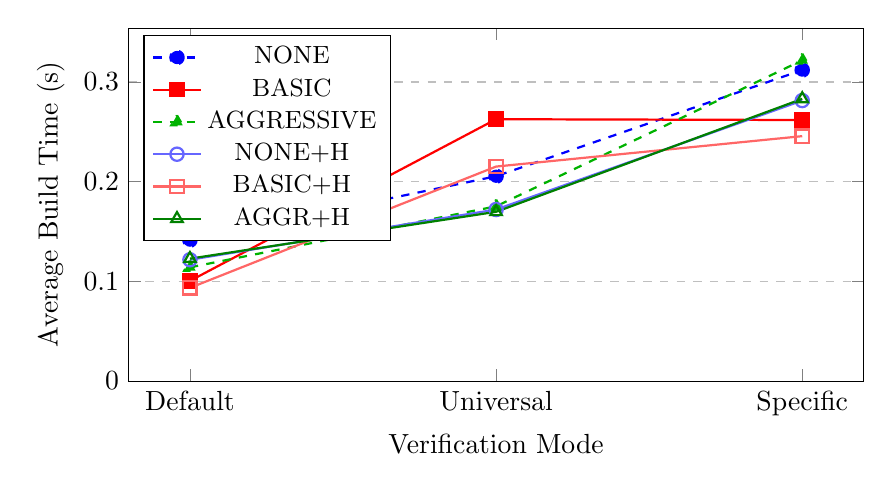
\begin{tikzpicture}
\begin{axis}[
    width=0.9\linewidth,
    height=0.5\linewidth,
    xlabel={Verification Mode},
    ylabel={Average Build Time (s)},
    symbolic x coords={Default,Universal,Specific},
    xtick=data,
    legend style={at={(0.02,0.98)}, anchor=north west, font=\small},
    ymajorgrids=true,
    grid style=dashed,
    ymin=0,
    mark options={scale=1.2}
]

\addplot[color=blue, mark=*, thick, dashed] coordinates {
    (Default,0.1414) (Universal,0.2055) (Specific,0.3120)
};
\addlegendentry{NONE}

\addplot[color=red, mark=square*, thick] coordinates {
    (Default,0.1005) (Universal,0.2627) (Specific,0.2619)
};
\addlegendentry{BASIC}

\addplot[color=green!70!black, mark=triangle*, thick, dashed] coordinates {
    (Default,0.1141) (Universal,0.1753) (Specific,0.3218)
};
\addlegendentry{AGGRESSIVE}

\addplot[color=blue!60, mark=o, thick] coordinates {
    (Default,0.1217) (Universal,0.1721) (Specific,0.2814)
};
\addlegendentry{NONE+H}

\addplot[color=red!60, mark=square, thick] coordinates {
    (Default,0.0935) (Universal,0.2152) (Specific,0.2457)
};
\addlegendentry{BASIC+H}

\addplot[color=green!50!black, mark=triangle, thick] coordinates {
    (Default,0.1228) (Universal,0.1698) (Specific,0.2831)
};
\addlegendentry{AGGR+H}

\end{axis}
\end{tikzpicture}
\caption{Average build times across verification modes. Default mode shows fastest build times; Specific mode has highest due to parameter processing overhead.}
\label{fig:build-time-modes}
\end{figure}

%% =============================================================================
\subsubsection*{Solve Time Analysis Across Verification Modes}
%% =============================================================================

\begin{figure}[H]
\centering
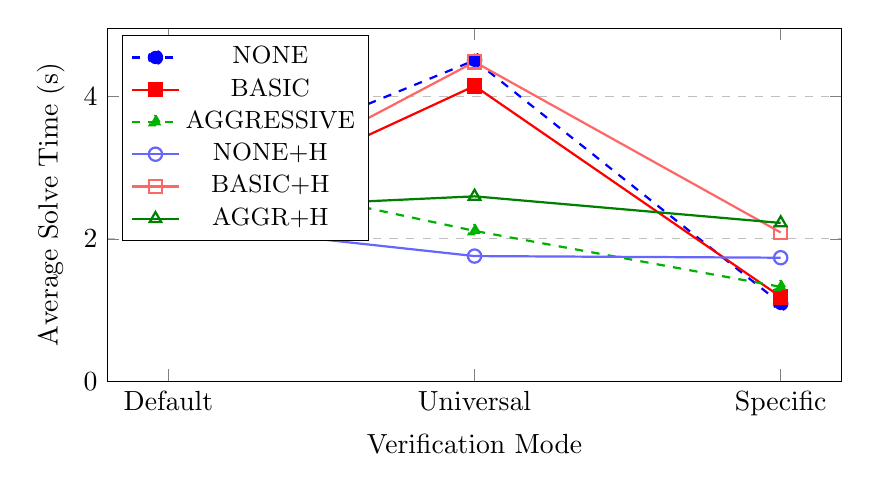
\begin{tikzpicture}
\begin{axis}[
    width=0.9\linewidth,
    height=0.5\linewidth,
    xlabel={Verification Mode},
    ylabel={Average Solve Time (s)},
    symbolic x coords={Default,Universal,Specific},
    xtick=data,
    legend style={at={(0.02,0.98)}, anchor=north west, font=\small},
    ymajorgrids=true,
    grid style=dashed,
    ymin=0,
    mark options={scale=1.2}
]

\addplot[color=blue, mark=*, thick, dashed] coordinates {
    (Default,2.7449) (Universal,4.5115) (Specific,1.0917)
};
\addlegendentry{NONE}

\addplot[color=red, mark=square*, thick] coordinates {
    (Default,2.1594) (Universal,4.1508) (Specific,1.1852)
};
\addlegendentry{BASIC}

\addplot[color=green!70!black, mark=triangle*, thick, dashed] coordinates {
    (Default,3.0309) (Universal,2.1122) (Specific,1.3254)
};
\addlegendentry{AGGRESSIVE}

\addplot[color=blue!60, mark=o, thick] coordinates {
    (Default,2.2272) (Universal,1.7583) (Specific,1.7351)
};
\addlegendentry{NONE+H}

\addplot[color=red!60, mark=square, thick] coordinates {
    (Default,2.2148) (Universal,4.4889) (Specific,2.0902)
};
\addlegendentry{BASIC+H}

\addplot[color=green!50!black, mark=triangle, thick] coordinates {
    (Default,2.3993) (Universal,2.5983) (Specific,2.2242)
};
\addlegendentry{AGGR+H}

\end{axis}
\end{tikzpicture}
\caption{Average solve times across verification modes. Universal mode exhibits highest solve times due to unconstrained initial states.}
\label{fig:solve-time-modes}
\end{figure}

%% =============================================================================
\subsubsection*{Build Time Analysis by Test Category}
%% =============================================================================

\begin{figure}[H]
\centering
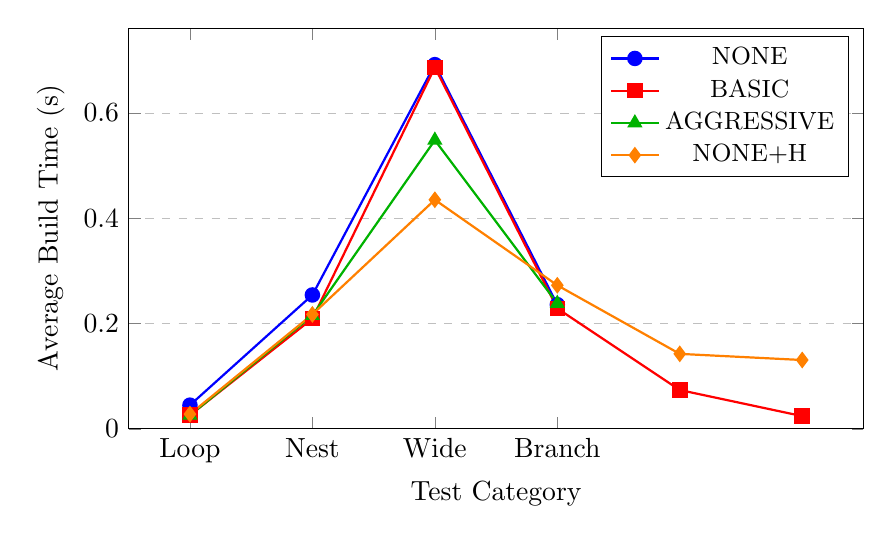
\begin{tikzpicture}
\begin{axis}[
    width=0.9\linewidth,
    height=0.55\linewidth,
    xlabel={Test Category},
    ylabel={Average Build Time (s)},
    symbolic x coords={Loop,Nest,Wide,Branch,Trig,Turn},
    xtick=data,
    legend style={at={(0.98,0.98)}, anchor=north east, font=\small},
    ymajorgrids=true,
    grid style=dashed,
    ymin=0,
    mark options={scale=1.2}
]

\addplot[color=blue, mark=*, thick] coordinates {
    (Loop,0.0449) (Nest,0.2543) (Wide,0.6920) (Branch,0.2359)
};
\addlegendentry{NONE}

\addplot[color=red, mark=square*, thick] coordinates {
    (Loop,0.0258) (Nest,0.2094) (Wide,0.6868) (Branch,0.2288) (Trig,0.0737) (Turn,0.0241)
};
\addlegendentry{BASIC}

\addplot[color=green!70!black, mark=triangle*, thick] coordinates {
    (Loop,0.0257) (Nest,0.2152) (Wide,0.5484) (Branch,0.2382)
};
\addlegendentry{AGGRESSIVE}

\addplot[color=orange, mark=diamond*, thick] coordinates {
    (Loop,0.0279) (Nest,0.2173) (Wide,0.4352) (Branch,0.2727) (Trig,0.1424) (Turn,0.1307)
};
\addlegendentry{NONE+H}

\end{axis}
\end{tikzpicture}
\caption{Average build times by test category (Default mode). Wide State tests have highest build times due to 8-dimensional state tracking.}
\label{fig:build-time-category}
\end{figure}

%% =============================================================================
\subsubsection*{Solve Time Analysis by Test Category}
%% =============================================================================

\begin{figure}[H]
\centering
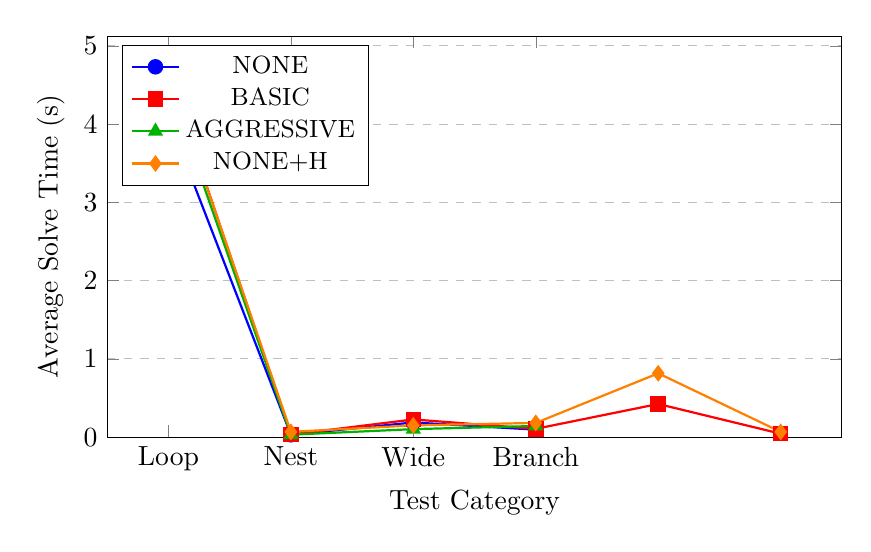
\begin{tikzpicture}
\begin{axis}[
    width=0.9\linewidth,
    height=0.55\linewidth,
    xlabel={Test Category},
    ylabel={Average Solve Time (s)},
    symbolic x coords={Loop,Nest,Wide,Branch,Trig,Turn},
    xtick=data,
    legend style={at={(0.02,0.98)}, anchor=north west, font=\small},
    ymajorgrids=true,
    grid style=dashed,
    ymin=0,
    mark options={scale=1.2}
]

\addplot[color=blue, mark=*, thick] coordinates {
    (Loop,4.0731) (Nest,0.0308) (Wide,0.1885) (Branch,0.0962)
};
\addlegendentry{NONE}

\addplot[color=red, mark=square*, thick] coordinates {
    (Loop,4.6524) (Nest,0.0333) (Wide,0.2266) (Branch,0.1070) (Trig,0.4244) (Turn,0.0444)
};
\addlegendentry{BASIC}

\addplot[color=green!70!black, mark=triangle*, thick] coordinates {
    (Loop,4.5010) (Nest,0.0319) (Wide,0.1030) (Branch,0.1433)
};
\addlegendentry{AGGRESSIVE}

\addplot[color=orange, mark=diamond*, thick] coordinates {
    (Loop,4.6291) (Nest,0.0682) (Wide,0.1510) (Branch,0.1824) (Trig,0.8161) (Turn,0.0675)
};
\addlegendentry{NONE+H}

\end{axis}
\end{tikzpicture}
\caption{Average solve times by test category (Default mode). Loop Scaling dominates due to tight bound invariant synthesis.}
\label{fig:solve-time-category}
\end{figure}

%% =============================================================================
\subsubsection*{Optimization Benefits}
%% =============================================================================

\begin{figure}[H]
\centering
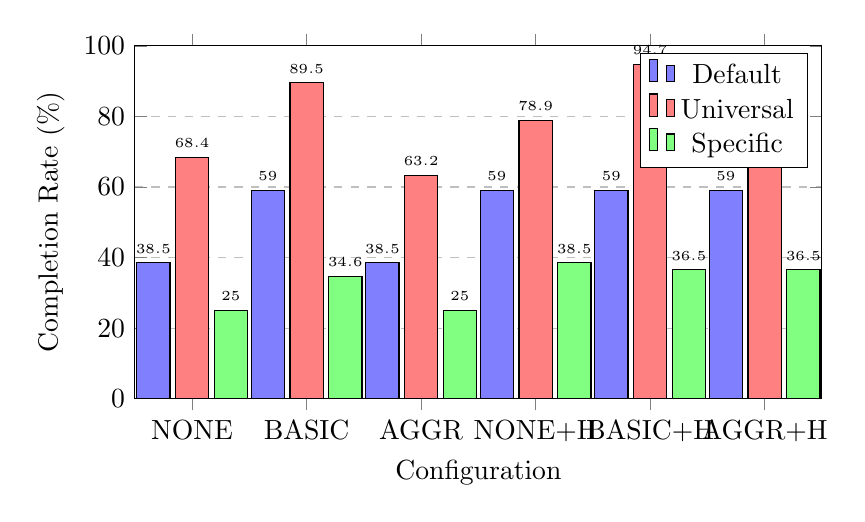
\begin{tikzpicture}
\begin{axis}[
    ybar,
    width=0.85\linewidth,
    height=0.5\linewidth,
    bar width=12pt,
    ymajorgrids=true,
    grid style=dashed,
    xlabel={Configuration},
    ylabel={Completion Rate (\%)},
    symbolic x coords={NONE,BASIC,AGGR,NONE+H,BASIC+H,AGGR+H},
    xtick=data,
    ymin=0, ymax=100,
    legend style={at={(0.98,0.98)}, anchor=north east},
    nodes near coords,
    nodes near coords align={vertical},
    every node near coord/.append style={font=\tiny}
]

\addplot[fill=blue!50] coordinates {
    (NONE,38.5) (BASIC,59.0) (AGGR,38.5) (NONE+H,59.0) (BASIC+H,59.0) (AGGR+H,59.0)
};
\addlegendentry{Default}

\addplot[fill=red!50] coordinates {
    (NONE,68.4) (BASIC,89.5) (AGGR,63.2) (NONE+H,78.9) (BASIC+H,94.7) (AGGR+H,81.6)
};
\addlegendentry{Universal}

\addplot[fill=green!50] coordinates {
    (NONE,25.0) (BASIC,34.6) (AGGR,25.0) (NONE+H,38.5) (BASIC+H,36.5) (AGGR+H,36.5)
};
\addlegendentry{Specific}

\end{axis}
\end{tikzpicture}
\caption{Test completion rates by configuration. \texttt{BASIC+H} achieves 94.7\% completion in Universal mode---the highest across all mode-configuration combinations.}
\label{fig:completion-by-opt}
\end{figure}

\begin{itemize}[leftmargin=1.5em]
    \item \textbf{\texttt{BASIC} provides consistent improvement.} In Default mode, completion jumps from 38.5\% (NONE) to 59.0\% (BASIC); in Universal mode, from 68.4\% to 89.5\%.
    \item \textbf{Mode-dependent behavior.} Universal mode shows the largest improvement with \texttt{BASIC} (68.4\% $\rightarrow$ 89.5\%), while Specific mode shows minimal benefit (25.0\% $\rightarrow$ 34.6\%).
\end{itemize}

%% =============================================================================
\subsubsection*{Hint Benifits}
%% =============================================================================

\subsubsection*{Timeout Reduction}

\begin{table}[H]
\centering
\caption{Timeout reduction rates with heading hints enabled.}
\label{tab:hint-reduction}
\begin{tabular}{lccc}
\toprule
\textbf{Mode} & \textbf{NONE $\rightarrow$ NONE+H} & \textbf{BASIC $\rightarrow$ BASIC+H} & \textbf{AGGR $\rightarrow$ AGGR+H} \\
\midrule
Default   & \textbf{33.3\%} (24$\rightarrow$16) & 0.0\% (16$\rightarrow$16)  & \textbf{33.3\%} (24$\rightarrow$16) \\
Universal & 33.3\% (12$\rightarrow$8) & \textbf{50.0\%} (4$\rightarrow$2) & \textbf{50.0\%} (14$\rightarrow$7) \\
Specific  & 17.9\% (39$\rightarrow$32) & 2.9\% (34$\rightarrow$33)  & 15.4\% (39$\rightarrow$33) \\
\bottomrule
\end{tabular}
\end{table}

% \begin{figure}[H]
% \centering
% \begin{tikzpicture}
% \begin{axis}[
%     ybar,
%     width=0.85\linewidth,
%     height=0.48\linewidth,
%     bar width=14pt,
%     ymajorgrids=true,
%     grid style=dashed,
%     xlabel={Optimization Level},
%     ylabel={Timeout Reduction (\%)},
%     symbolic x coords={NONE,BASIC,AGGRESSIVE},
%     xtick=data,
%     ymin=0, ymax=60,
%     legend style={at={(0.98,0.98)}, anchor=north east},
%     nodes near coords,
%     nodes near coords align={vertical},
%     every node near coord/.append style={font=\small}
% ]

% \addplot[fill=blue!50] coordinates {
%     (NONE,33.3) (BASIC,0.0) (AGGRESSIVE,33.3)
% };
% \addlegendentry{Default}

% \addplot[fill=red!50] coordinates {
%     (NONE,33.3) (BASIC,50.0) (AGGRESSIVE,50.0)
% };
% \addlegendentry{Universal}

% \addplot[fill=green!50] coordinates {
%     (NONE,17.9) (BASIC,2.9) (AGGRESSIVE,15.4)
% };
% \addlegendentry{Specific}

% \end{axis}
% \end{tikzpicture}
% \caption{Timeout reduction rates when hints are enabled. Universal mode sees 50\% reduction for BASIC and AGGRESSIVE configurations.}
% \label{fig:hint-reduction}
% \end{figure}

\subsubsection*{Tests Uniquely Solved by Hints}

\begin{table}[H]
\centering
\caption{Number of tests uniquely solved when hints are enabled (timeout$\rightarrow$success).}
\label{tab:hint-unique}
\begin{tabular}{lccc}
\toprule
\textbf{Mode} & \textbf{NONE} & \textbf{BASIC} & \textbf{AGGRESSIVE} \\
\midrule
Default   &  8 & 1 &  8 \\
Universal &  5 & 2 &  7 \\
Specific  &  7 & 2 &  6 \\
\midrule
\textbf{Total} & \textbf{20} & \textbf{5} & \textbf{21} \\
\bottomrule
\end{tabular}
\end{table}


\begin{itemize}[leftmargin=1.5em, nosep]
    \item \textbf{Hints are most effective with \texttt{NONE} and \texttt{AGGRESSIVE}.} These configurations benefit from 33\% timeout reduction in Default mode and up to 50\% in Universal mode.
    
    \item \textbf{Combined \texttt{BASIC+H} is optimal.} It achieves the highest completion rates (59.0\% Default, 94.7\% Universal, 36.5\% Specific).
\end{itemize}

%% =============================================================================
\subsubsection*{Overall Performance}
%% =============================================================================


\begin{figure}[H]
\centering
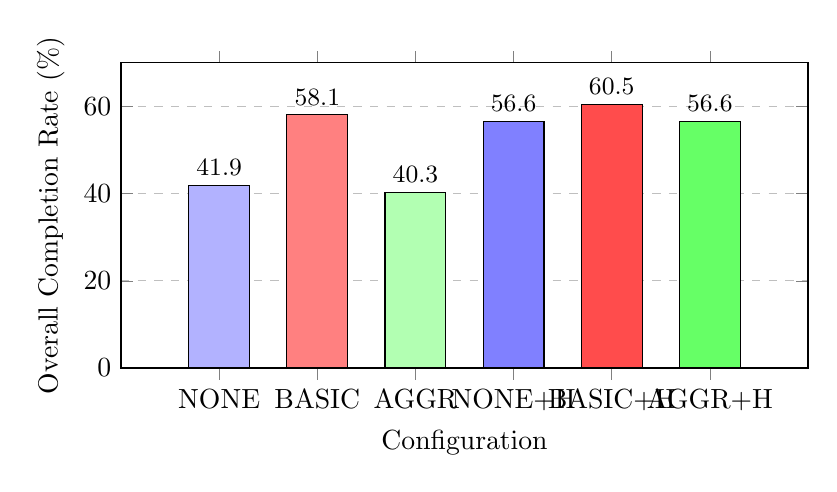
\begin{tikzpicture}
\begin{axis}[
    ybar=0pt,
    bar width=22pt,
    width=0.85\linewidth,
    height=0.45\linewidth,
    ymajorgrids=true,
    grid style=dashed,
    xlabel={Configuration},
    ylabel={Overall Completion Rate (\%)},
    xtick={1,2,3,4,5,6},
    xticklabels={NONE,BASIC,AGGR,NONE+H,BASIC+H,AGGR+H},
    xmin=0, xmax=7,
    ymin=0, ymax=70,
    nodes near coords,
    every node near coord/.append style={font=\small},
]
\addplot[ybar, bar shift=0pt, fill=blue!30,  draw=black] coordinates {(1,41.9)};
\addplot[ybar, bar shift=0pt, fill=red!50,   draw=black] coordinates {(2,58.1)};
\addplot[ybar, bar shift=0pt, fill=green!30, draw=black] coordinates {(3,40.3)};
\addplot[ybar, bar shift=0pt, fill=blue!50,  draw=black] coordinates {(4,56.6)};
\addplot[ybar, bar shift=0pt, fill=red!70,   draw=black] coordinates {(5,60.5)};
\addplot[ybar, bar shift=0pt, fill=green!60, draw=black] coordinates {(6,56.6)};
\end{axis}
\end{tikzpicture}
\caption{Overall completion rates across all 129 tests. \texttt{BASIC+H} achieves the highest overall rate (60.5\%).}
\label{fig:overall-completion}
\end{figure}

Based on the empirical analysis:

\begin{enumerate}[leftmargin=1.5em]
    \item \textbf{Use \texttt{BASIC} optimization as default.} It provides the best balance of build time reduction (1.41$\times$ speedup) and completion rate improvement (38.5\% $\rightarrow$ 59.0\% in Default mode).
    
    \item \textbf{Enable hints for trigonometric programs.} When verifying programs with heading-dependent motion (\texttt{forward}/\texttt{backward}), hints provide 33--50\% timeout reduction.
\end{enumerate}

\subsection*{Running the Performance Tests}

\begin{lstlisting}[style=terminal, language=bash]
cd Chiron-Framework/ChironCore/CHC_Verification/performance_tests
pytest test_default.py -v      # Default mode benchmarks
pytest test_universal.py -v    # Universal mode benchmarks
pytest test_specific.py -v     # Specific mode benchmarks
\end{lstlisting}

\noindent Results are written to \texttt{perf\_results\_<mode>.csv} for analysis.